\documentclass[a4paper,12pt,oneside]{book}
\usepackage[italian]{babel}
\usepackage[utf8]{inputenc}
\usepackage{textcomp}
\usepackage[parfill]{parskip} %Se necessatrio non indenta, ma inserisce spazio
\usepackage{graphicx}
\usepackage{hyperref}
\usepackage{amsmath} %To number equations

\usepackage{titling}
\newcommand{\subtitle}[1]{%
 \posttitle{%
 \par\end{center}
 \begin{center}\large#1\end{center}
 \vskip6.5em}%
}

\author{Andrea Onofri e Dario Sacco}
\date{Update: v. 1.0 (15/03/2021), compil. 2021-04-27}
\title{Metodologia sperimentale per le scienze agrarie}
\subtitle{}


%***************************************************************

%Specific RMarkdown
\usepackage{color}
\usepackage{fancyvrb}
\usepackage{longtable}
\usepackage{booktabs}
\providecommand{\tightlist}{%
  \setlength{\itemsep}{0pt}\setlength{\parskip}{0pt}}
\newcommand{\VerbBar}{|}
\newcommand{\VERB}{\Verb[commandchars=\\\{\}]}
\DefineVerbatimEnvironment{Highlighting}{Verbatim}{commandchars=\\\{\},fontsize=\small}
\usepackage{framed}
%\newenvironment{Shaded}{}{}
\newenvironment{Shaded}{\begin{snugshade}}{\end{snugshade}}
\definecolor{shadecolor}{RGB}{250,248,248}
\newcommand{\KeywordTok}[1]{#1}
\newcommand{\DataTypeTok}[1]{#1}
\newcommand{\DecValTok}[1]{#1}
\newcommand{\BaseNTok}[1]{#1}
\newcommand{\FloatTok}[1]{#1}
\newcommand{\ConstantTok}[1]{#1}
\newcommand{\CharTok}[1]{#1}
\newcommand{\SpecialCharTok}[1]{#1}
\newcommand{\StringTok}[1]{#1}
\newcommand{\VerbatimStringTok}[1]{#1}
\newcommand{\SpecialStringTok}[1]{#1}
\newcommand{\ImportTok}[1]{#1}
\newcommand{\CommentTok}[1]{#1}
\newcommand{\DocumentationTok}[1]{#1}
\newcommand{\AnnotationTok}[1]{#1}
\newcommand{\CommentVarTok}[1]{#1}
\newcommand{\OtherTok}[1]{#1}
\newcommand{\FunctionTok}[1]{#1}
\newcommand{\VariableTok}[1]{#1}
\newcommand{\ControlFlowTok}[1]{#1}
\newcommand{\OperatorTok}[1]{#1}
\newcommand{\BuiltInTok}[1]{#1}
\newcommand{\ExtensionTok}[1]{#1}
\newcommand{\PreprocessorTok}[1]{#1}
\newcommand{\AttributeTok}[1]{#1}
\newcommand{\RegionMarkerTok}[1]{#1}
\newcommand{\InformationTok}[1]{#1}
\newcommand{\WarningTok}[1]{#1}
\newcommand{\AlertTok}[1]{#1}
\newcommand{\ErrorTok}[1]{#1}
\newcommand{\NormalTok}[1]{#1}
% Redefine \includegraphics so that, unless explicit options are
% given, the image width will not exceed the width of the page.
% Images get their normal width if they fit onto the page, but
% are scaled down if they would overflow the margins.

\begin{document}

\maketitle
\tableofcontents

\hypertarget{premessa}{%
\chapter*{Premessa}\label{premessa}}
\addcontentsline{toc}{chapter}{Premessa}

Placeholder

\hypertarget{obiettivi}{%
\section*{Obiettivi}\label{obiettivi}}
\addcontentsline{toc}{section}{Obiettivi}

\hypertarget{organizzazione}{%
\section*{Organizzazione}\label{organizzazione}}
\addcontentsline{toc}{section}{Organizzazione}

\hypertarget{software-statistico}{%
\section*{Software statistico}\label{software-statistico}}
\addcontentsline{toc}{section}{Software statistico}

\hypertarget{the-authors}{%
\section*{The authors}\label{the-authors}}
\addcontentsline{toc}{section}{The authors}

\hypertarget{ringraziamenti}{%
\section*{Ringraziamenti}\label{ringraziamenti}}
\addcontentsline{toc}{section}{Ringraziamenti}

\hypertarget{scienza-e-pseudo-scienza}{%
\chapter{Scienza e pseudo-scienza}\label{scienza-e-pseudo-scienza}}

Placeholder

\hypertarget{scienza-dati}{%
\section{Scienza = dati}\label{scienza-dati}}

\hypertarget{dati-buoni-e-cattivi}{%
\section{Dati `buoni' e `cattivi'}\label{dati-buoni-e-cattivi}}

\hypertarget{dati-buoni-e-metodi-buoni}{%
\section{Dati `buoni' e metodi `buoni'}\label{dati-buoni-e-metodi-buoni}}

\hypertarget{il-principio-di-falsificazione}{%
\section{Il principio di falsificazione}\label{il-principio-di-falsificazione}}

\hypertarget{falsificare-un-risultato}{%
\section{Falsificare un risultato}\label{falsificare-un-risultato}}

\hypertarget{elementi-fondamentali-del-disegno-sperimentale}{%
\section{Elementi fondamentali del disegno sperimentale}\label{elementi-fondamentali-del-disegno-sperimentale}}

\hypertarget{controllo-degli-errori}{%
\subsection{Controllo degli errori}\label{controllo-degli-errori}}

\hypertarget{replicazione}{%
\subsection{Replicazione}\label{replicazione}}

\hypertarget{randomizzazione}{%
\subsection{Randomizzazione}\label{randomizzazione}}

\hypertarget{esperimenti-invalidi}{%
\subsection{Esperimenti invalidi}\label{esperimenti-invalidi}}

\hypertarget{cattivo-controllo-degli-errori}{%
\subsubsection{Cattivo controllo degli errori}\label{cattivo-controllo-degli-errori}}

\hypertarget{confounding-e-correlazione-spuria}{%
\subsubsection{`Confounding' e correlazione spuria}\label{confounding-e-correlazione-spuria}}

\hypertarget{pseudo-repliche-e-randomizzazione-poco-attenta}{%
\subsubsection{Pseudo-repliche e randomizzazione poco attenta}\label{pseudo-repliche-e-randomizzazione-poco-attenta}}

\hypertarget{chi-valuta-se-un-esperimento-uxe8-attendibile}{%
\section{Chi valuta se un esperimento è attendibile?}\label{chi-valuta-se-un-esperimento-uxe8-attendibile}}

\hypertarget{conclusioni}{%
\section{Conclusioni}\label{conclusioni}}

\hypertarget{altre-letture}{%
\section{Altre letture}\label{altre-letture}}

\hypertarget{progettare-un-esperimento}{%
\chapter{Progettare un esperimento}\label{progettare-un-esperimento}}

Placeholder

\hypertarget{gli-elementi-della-ricerca}{%
\section{Gli elementi della ricerca}\label{gli-elementi-della-ricerca}}

\hypertarget{ipotesi-scientifica-rightarrow-obiettivo-dellesperimento}{%
\section{\texorpdfstring{Ipotesi scientifica \(\rightarrow\) obiettivo dell'esperimento}{Ipotesi scientifica \textbackslash rightarrow obiettivo dell'esperimento}}\label{ipotesi-scientifica-rightarrow-obiettivo-dellesperimento}}

\hypertarget{identificazione-dei-fattori-sperimentali}{%
\section{Identificazione dei fattori sperimentali}\label{identificazione-dei-fattori-sperimentali}}

\hypertarget{esperimenti-multi-fattoriali}{%
\subsection{Esperimenti (multi-)fattoriali}\label{esperimenti-multi-fattoriali}}

\hypertarget{controllo-o-testimone}{%
\subsection{Controllo o testimone}\label{controllo-o-testimone}}

\hypertarget{le-unituxe0-sperimentali}{%
\section{Le unità sperimentali}\label{le-unituxe0-sperimentali}}

\hypertarget{allocazione-dei-trattamenti}{%
\section{Allocazione dei trattamenti}\label{allocazione-dei-trattamenti}}

\hypertarget{le-variabili-sperimentali}{%
\section{Le variabili sperimentali}\label{le-variabili-sperimentali}}

\hypertarget{variabili-nominali-categoriche}{%
\subsection{Variabili nominali (categoriche)}\label{variabili-nominali-categoriche}}

\hypertarget{variabili-ordinali}{%
\subsection{Variabili ordinali}\label{variabili-ordinali}}

\hypertarget{variabili-quantitative-discrete}{%
\subsection{Variabili quantitative discrete}\label{variabili-quantitative-discrete}}

\hypertarget{variabili-quantitative-continue}{%
\subsection{Variabili quantitative continue}\label{variabili-quantitative-continue}}

\hypertarget{rilievi-visivi-e-sensoriali}{%
\subsection{Rilievi visivi e sensoriali}\label{rilievi-visivi-e-sensoriali}}

\hypertarget{variabili-di-confondimento}{%
\subsection{Variabili di confondimento}\label{variabili-di-confondimento}}

\hypertarget{esperimenti-di-campo}{%
\section{Esperimenti di campo}\label{esperimenti-di-campo}}

\hypertarget{scegliere-il-campo}{%
\subsection{Scegliere il campo}\label{scegliere-il-campo}}

\hypertarget{le-unituxe0-sperimentali-in-campo}{%
\subsection{Le unità sperimentali in campo}\label{le-unituxe0-sperimentali-in-campo}}

\hypertarget{numero-di-repliche}{%
\subsection{Numero di repliche}\label{numero-di-repliche}}

\hypertarget{la-mappa-di-campo}{%
\subsection{La mappa di campo}\label{la-mappa-di-campo}}

\hypertarget{lay-out-sperimentale}{%
\subsection{Lay-out sperimentale}\label{lay-out-sperimentale}}

\hypertarget{disegni-completamente-randomizzati}{%
\subsubsection{Disegni completamente randomizzati}\label{disegni-completamente-randomizzati}}

\hypertarget{disegni-a-blocchi-randomizzati}{%
\subsubsection{Disegni a blocchi randomizzati}\label{disegni-a-blocchi-randomizzati}}

\hypertarget{disegni-a-quadrato-latino}{%
\subsubsection{Disegni a quadrato latino}\label{disegni-a-quadrato-latino}}

\hypertarget{disegni-a-split-plot}{%
\subsubsection{Disegni a split-plot}\label{disegni-a-split-plot}}

\hypertarget{disegni-a-strip-plot}{%
\subsubsection{Disegni a strip-plot}\label{disegni-a-strip-plot}}

\hypertarget{altre-letture-1}{%
\section{Altre letture}\label{altre-letture-1}}

\hypertarget{richiami-di-statistica-descrittiva}{%
\chapter{Richiami di statistica descrittiva}\label{richiami-di-statistica-descrittiva}}

Placeholder

\hypertarget{dati-quantitativi}{%
\section{Dati quantitativi}\label{dati-quantitativi}}

\hypertarget{indicatori-di-tendenza-centrale}{%
\subsection{Indicatori di tendenza centrale}\label{indicatori-di-tendenza-centrale}}

\hypertarget{indicatori-di-dispersione}{%
\subsection{Indicatori di dispersione}\label{indicatori-di-dispersione}}

\hypertarget{incertezza-delle-misure-derivate}{%
\subsection{Incertezza delle misure derivate}\label{incertezza-delle-misure-derivate}}

\hypertarget{relazioni-tra-variabili-quantitative-correlazione}{%
\subsection{Relazioni tra variabili quantitative: correlazione}\label{relazioni-tra-variabili-quantitative-correlazione}}

\hypertarget{dati-qualitativi}{%
\section{Dati qualitativi}\label{dati-qualitativi}}

\hypertarget{distribuzioni-di-frequenze-e-classamento}{%
\subsection{Distribuzioni di frequenze e classamento}\label{distribuzioni-di-frequenze-e-classamento}}

\hypertarget{statistiche-descrittive-per-le-distribuzioni-di-frequenze}{%
\subsection{Statistiche descrittive per le distribuzioni di frequenze}\label{statistiche-descrittive-per-le-distribuzioni-di-frequenze}}

\hypertarget{distribuzioni-di-frequenza-bivariate-le-tabelle-di-contingenze}{%
\subsection{Distribuzioni di frequenza bivariate: le tabelle di contingenze}\label{distribuzioni-di-frequenza-bivariate-le-tabelle-di-contingenze}}

\hypertarget{connessione}{%
\subsection{Connessione}\label{connessione}}

\hypertarget{statistiche-descrittive-con-r}{%
\section{Statistiche descrittive con R}\label{statistiche-descrittive-con-r}}

\hypertarget{descrizione-dei-sottogruppi}{%
\subsection{Descrizione dei sottogruppi}\label{descrizione-dei-sottogruppi}}

\hypertarget{distribuzioni-di-frequenze-e-classamento-1}{%
\subsection{Distribuzioni di frequenze e classamento}\label{distribuzioni-di-frequenze-e-classamento-1}}

\hypertarget{connessione-1}{%
\subsection{Connessione}\label{connessione-1}}

\hypertarget{altre-letture-2}{%
\section{Altre letture}\label{altre-letture-2}}

\hypertarget{modelli-statistici-ed-analisi-dei-dati}{%
\chapter{Modelli statistici ed analisi dei dati}\label{modelli-statistici-ed-analisi-dei-dati}}

Placeholder

\hypertarget{verituxe0-vera-e-modelli-deterministici}{%
\section{Verità `vera' e modelli deterministici}\label{verituxe0-vera-e-modelli-deterministici}}

\hypertarget{genesi-deterministica-delle-osservazioni-sperimentali}{%
\section{Genesi deterministica delle osservazioni sperimentali}\label{genesi-deterministica-delle-osservazioni-sperimentali}}

\hypertarget{errore-sperimentale-e-modelli-stocastici}{%
\section{Errore sperimentale e modelli stocastici}\label{errore-sperimentale-e-modelli-stocastici}}

\hypertarget{funzioni-di-probabilituxe0}{%
\subsection{Funzioni di probabilità}\label{funzioni-di-probabilituxe0}}

\hypertarget{funzioni-di-densituxe0}{%
\subsection{Funzioni di densità}\label{funzioni-di-densituxe0}}

\hypertarget{la-distribuzione-normale-curva-di-gauss}{%
\subsection{La distribuzione normale (curva di Gauss)}\label{la-distribuzione-normale-curva-di-gauss}}

\hypertarget{modelli-a-due-facce}{%
\section{Modelli `a due facce'}\label{modelli-a-due-facce}}

\hypertarget{e-allora}{%
\section{E allora?}\label{e-allora}}

\hypertarget{le-simulazioni-monte-carlo}{%
\section{Le simulazioni Monte Carlo}\label{le-simulazioni-monte-carlo}}

\hypertarget{analisi-dei-dati-e-model-fitting}{%
\section{Analisi dei dati e `model fitting'}\label{analisi-dei-dati-e-model-fitting}}

\hypertarget{modelli-stocastici-non-normali}{%
\section{Modelli stocastici non-normali}\label{modelli-stocastici-non-normali}}

\hypertarget{altre-letture-3}{%
\section{Altre letture}\label{altre-letture-3}}

\hypertarget{stime-ed-incertezza}{%
\chapter{Stime ed incertezza}\label{stime-ed-incertezza}}

Placeholder

\hypertarget{esempio-una-soluzione-erbicida}{%
\section{Esempio: una soluzione erbicida}\label{esempio-una-soluzione-erbicida}}

\hypertarget{analisi-dei-dati-stima-dei-parametri}{%
\subsection{Analisi dei dati: stima dei parametri}\label{analisi-dei-dati-stima-dei-parametri}}

\hypertarget{la-sampling-distribution}{%
\subsection{La `sampling distribution'}\label{la-sampling-distribution}}

\hypertarget{lerrore-standard}{%
\subsection{L'errore standard}\label{lerrore-standard}}

\hypertarget{stima-per-intervallo}{%
\section{Stima per intervallo}\label{stima-per-intervallo}}

\hypertarget{lintervallo-di-confidenza}{%
\section{L'intervallo di confidenza}\label{lintervallo-di-confidenza}}

\hypertarget{qual-uxe8-il-senso-dellintervallo-di-confidenza}{%
\section{Qual è il senso dell'intervallo di confidenza?}\label{qual-uxe8-il-senso-dellintervallo-di-confidenza}}

\hypertarget{come-presentare-i-risultati-degli-esperimenti}{%
\section{Come presentare i risultati degli esperimenti}\label{come-presentare-i-risultati-degli-esperimenti}}

\hypertarget{alcune-precisazioni}{%
\section{Alcune precisazioni}\label{alcune-precisazioni}}

\hypertarget{campioni-numerosi-e-non}{%
\subsection{Campioni numerosi e non}\label{campioni-numerosi-e-non}}

\hypertarget{popolazioni-gaussiane-e-non}{%
\subsection{Popolazioni gaussiane e non}\label{popolazioni-gaussiane-e-non}}

\hypertarget{analisi-statistica-dei-dati-riassunto-del-percorso-logico}{%
\section{Analisi statistica dei dati: riassunto del percorso logico}\label{analisi-statistica-dei-dati-riassunto-del-percorso-logico}}

\hypertarget{da-ricordare}{%
\section{Da ricordare}\label{da-ricordare}}

\hypertarget{per-approfondire-un-po}{%
\section{Per approfondire un po'\ldots{}}\label{per-approfondire-un-po}}

\hypertarget{coverage-degli-intervalli-di-confidenza}{%
\section{\texorpdfstring{\emph{Coverage} degli intervalli di confidenza}{Coverage degli intervalli di confidenza}}\label{coverage-degli-intervalli-di-confidenza}}

\hypertarget{intervalli-di-confidenza-per-fenomeni-non-normali}{%
\subsection{Intervalli di confidenza per fenomeni non-normali}\label{intervalli-di-confidenza-per-fenomeni-non-normali}}

\hypertarget{altre-letture-4}{%
\section{Altre letture}\label{altre-letture-4}}

\hypertarget{decisioni-ed-incertezza}{%
\chapter{Decisioni ed incertezza}\label{decisioni-ed-incertezza}}

Placeholder

\hypertarget{confronto-tra-due-medie-il-test-t-di-student}{%
\section{Confronto tra due medie: il test t di Student}\label{confronto-tra-due-medie-il-test-t-di-student}}

\hypertarget{lipotesi-nulla-e-alternativa}{%
\subsection{L'ipotesi nulla e alternativa}\label{lipotesi-nulla-e-alternativa}}

\hypertarget{la-statistica-t}{%
\subsection{La statistica T}\label{la-statistica-t}}

\hypertarget{simulazione-monte-carlo}{%
\subsection{Simulazione Monte Carlo}\label{simulazione-monte-carlo}}

\hypertarget{soluzione-formale}{%
\subsection{Soluzione formale}\label{soluzione-formale}}

\hypertarget{interpretazione-del-p-level}{%
\subsection{Interpretazione del P-level}\label{interpretazione-del-p-level}}

\hypertarget{tipologie-alternative-di-test-t-di-student}{%
\subsection{Tipologie alternative di test t di Student}\label{tipologie-alternative-di-test-t-di-student}}

\hypertarget{confronto-tra-due-proporzioni-il-test-chi2}{%
\section{\texorpdfstring{Confronto tra due proporzioni: il test \(\chi^2\)}{Confronto tra due proporzioni: il test \textbackslash chi\^{}2}}\label{confronto-tra-due-proporzioni-il-test-chi2}}

\hypertarget{simulazione-monte-carlo-1}{%
\subsection{Simulazione Monte Carlo}\label{simulazione-monte-carlo-1}}

\hypertarget{soluzione-formale-1}{%
\subsection{Soluzione formale}\label{soluzione-formale-1}}

\hypertarget{conclusioni-e-riepilogo}{%
\section{Conclusioni e riepilogo}\label{conclusioni-e-riepilogo}}

\hypertarget{altre-letture-5}{%
\section{Altre letture}\label{altre-letture-5}}

\hypertarget{modelli-anova-ad-una-via}{%
\chapter{Modelli ANOVA ad una via}\label{modelli-anova-ad-una-via}}

Placeholder

\hypertarget{caso-studio-confronto-tra-erbicidi-in-vaso}{%
\section{Caso-studio: confronto tra erbicidi in vaso}\label{caso-studio-confronto-tra-erbicidi-in-vaso}}

\hypertarget{descrizione-del-dataset}{%
\section{Descrizione del dataset}\label{descrizione-del-dataset}}

\hypertarget{definizione-di-un-modello-lineare}{%
\section{Definizione di un modello lineare}\label{definizione-di-un-modello-lineare}}

\hypertarget{parametrizzazione-del-modello}{%
\section{Parametrizzazione del modello}\label{parametrizzazione-del-modello}}

\hypertarget{assunzioni-di-base}{%
\section{Assunzioni di base}\label{assunzioni-di-base}}

\hypertarget{fitting-del-modello-metodo-manuale}{%
\section{Fitting del modello: metodo manuale}\label{fitting-del-modello-metodo-manuale}}

\hypertarget{stima-dei-parametri}{%
\subsection{Stima dei parametri}\label{stima-dei-parametri}}

\hypertarget{calcolo-dei-residui}{%
\subsection{Calcolo dei residui}\label{calcolo-dei-residui}}

\hypertarget{stima-di-sigma}{%
\subsection{\texorpdfstring{Stima di \(\sigma\)}{Stima di \textbackslash sigma}}\label{stima-di-sigma}}

\hypertarget{scomposizione-della-varianza}{%
\section{Scomposizione della varianza}\label{scomposizione-della-varianza}}

\hypertarget{test-dipotesi}{%
\section{Test d'ipotesi}\label{test-dipotesi}}

\hypertarget{inferenza-statistica}{%
\section{Inferenza statistica}\label{inferenza-statistica}}

\hypertarget{fitting-del-modello-con-r}{%
\section{Fitting del modello con R}\label{fitting-del-modello-con-r}}

\hypertarget{medie-marginali-attese}{%
\section{Medie marginali attese}\label{medie-marginali-attese}}

\hypertarget{per-concludere}{%
\section{Per concludere \ldots{}}\label{per-concludere}}

\hypertarget{altre-letture-6}{%
\section{Altre letture}\label{altre-letture-6}}

\hypertarget{la-verifica-delle-assunzioni-di-base}{%
\chapter{La verifica delle assunzioni di base}\label{la-verifica-delle-assunzioni-di-base}}

Placeholder

\hypertarget{violazioni-delle-assunzioni-di-base}{%
\section{Violazioni delle assunzioni di base}\label{violazioni-delle-assunzioni-di-base}}

\hypertarget{procedure-diagnostiche}{%
\section{Procedure diagnostiche}\label{procedure-diagnostiche}}

\hypertarget{analisi-grafica-dei-residui}{%
\section{Analisi grafica dei residui}\label{analisi-grafica-dei-residui}}

\hypertarget{grafico-dei-residui-contro-i-valori-attesi}{%
\subsection{Grafico dei residui contro i valori attesi}\label{grafico-dei-residui-contro-i-valori-attesi}}

\hypertarget{qq-plot}{%
\subsection{QQ-plot}\label{qq-plot}}

\hypertarget{test-dipotesi-1}{%
\section{Test d'ipotesi}\label{test-dipotesi-1}}

\hypertarget{risultati-contraddittori}{%
\section{Risultati contraddittori}\label{risultati-contraddittori}}

\hypertarget{terapia}{%
\section{`Terapia'}\label{terapia}}

\hypertarget{correzionerimozione-degli-outliers}{%
\subsection{Correzione/Rimozione degli outliers}\label{correzionerimozione-degli-outliers}}

\hypertarget{correzione-del-modello}{%
\subsection{Correzione del modello}\label{correzione-del-modello}}

\hypertarget{trasformazione-della-variabile-indipendente}{%
\subsection{Trasformazione della variabile indipendente}\label{trasformazione-della-variabile-indipendente}}

\hypertarget{impiego-di-metodiche-statistiche-avanzate}{%
\subsection{Impiego di metodiche statistiche avanzate}\label{impiego-di-metodiche-statistiche-avanzate}}

\hypertarget{trasformazioni-stabilizzanti}{%
\subsection{Trasformazioni stabilizzanti}\label{trasformazioni-stabilizzanti}}

\hypertarget{esempio-1}{%
\section{Esempio 1}\label{esempio-1}}

\hypertarget{esempio-2}{%
\section{Esempio 2}\label{esempio-2}}

\hypertarget{altre-letture-7}{%
\section{Altre letture}\label{altre-letture-7}}

\hypertarget{contrasti-e-confronti-multipli}{%
\chapter{Contrasti e confronti multipli}\label{contrasti-e-confronti-multipli}}

Placeholder

\hypertarget{esempio}{%
\section{Esempio}\label{esempio}}

\hypertarget{i-contrasti}{%
\section{I contrasti}\label{i-contrasti}}

\hypertarget{i-contrasti-con-r}{%
\section{I contrasti con R}\label{i-contrasti-con-r}}

\hypertarget{i-confronti-multipli-a-coppie-pairwise-comparisons}{%
\section{I confronti multipli a coppie (pairwise comparisons)}\label{i-confronti-multipli-a-coppie-pairwise-comparisons}}

\hypertarget{display-a-lettere}{%
\section{Display a lettere}\label{display-a-lettere}}

\hypertarget{tassi-di-errore-per-confronto-e-per-esperimento}{%
\section{Tassi di errore per confronto e per esperimento}\label{tassi-di-errore-per-confronto-e-per-esperimento}}

\hypertarget{aggiustamento-per-la-molteplicituxe0}{%
\section{Aggiustamento per la molteplicità}\label{aggiustamento-per-la-molteplicituxe0}}

\hypertarget{e-le-classiche-procedure-di-confronto-multiplo}{%
\section{E le classiche procedure di confronto multiplo?}\label{e-le-classiche-procedure-di-confronto-multiplo}}

\hypertarget{consigli-pratici}{%
\section{Consigli pratici}\label{consigli-pratici}}

\hypertarget{altre-letture-8}{%
\section{Altre letture}\label{altre-letture-8}}

\hypertarget{modelli-anova-con-fattori-di-blocco}{%
\chapter{Modelli ANOVA con fattori di blocco}\label{modelli-anova-con-fattori-di-blocco}}

Nel capitolo 7 abbiamo impiegato un modello ANOVA con una sola variabile indipendente categorica, assumendo che le unità sperimentali, escluso l'effetto del trattamento, fossero totalmente indipendenti tra di loro. Questa assunzione era totalmente realistica, poiché si trattava di un disegno sperimentale a randomizzazione completa, dove non sussistevano raggruppamenti di alcun tipo, escluso quello dettato dal trattamento in studio.

Se invece l'esperimento include uno o più \emph{blocking factors}, le osservazioni che appartengono allo stesso blocco sono più simila tra loro delle osservazioni che appartengono a blocchi diversi, proprio perché condividono le condizioni del blocco stesso. Per non invalidare l'indipendenza dei residui dobbiamo definire un modello ANOVA che tenga conto anche dei fattori di raggruppamento, in modo che il loro effetto non sia trascurato e, di conseguenza, si sommi agli effetti residui. Come al solito, affrontiamo questo tema partendo da alcuni esempi pratici.

\hypertarget{caso-studio-confronto-tra-erbicidi-in-campo}{%
\section{Caso-studio: confronto tra erbicidi in campo}\label{caso-studio-confronto-tra-erbicidi-in-campo}}

Abbiamo una prova di confronto tra erbicidi in mais, con 13 formulati, due testimoni inerbiti (che, per comodità, considereremo due trattamenti diversi) e un testimone scerbato. Al momento di impiantare la prova, era lecito ipotizzare che, pur scegliendo un appezzamento il più omogeneo possibile, avremmo potuto riscontrare differenze di infestazione tra un punto e l'altro del campo, con un presumibile gradiente procedendo dai lati (vicino alle fosse) verso il centro. In questa situazione, se l'esperimento fosse stato disegnato a randomizzazione completa, le differenze di infestazione tra una parte e l'altra del campo sarebbero state trascurate e avrebbero finito per incrementare l'errore sperimentale, diminuendo l'efficienza dell'esperimento.

Abbiamo quindi impiegato un disegno a blocchi randomizzati con quattro repliche; il campo è stato suddiviso in tante sezioni (dette blocchi) quante erano le repliche (quattro), perpendicolarmente al gradiente di infestazione trasversale. In questo modo, l'ambiente era relativamente omogeneo all'interno di ciascun blocco, nel quale è stata collocata una replica per trattamento.

Il dataset dei risultati (`rimsulfuron.csv') è disponibile nella solita \emph{repository} online. Nel box sottostante, carichiamo il file e trasformiamo le due variabili esplicative (blocco e trattamento) in fattori sperimentali. Più sotto, mostriamo la tabella in formato `WIDE' (una riga per trattamento, con le repliche sulle colonne), con le medie di riga (trattamento) e di colonna (blocco)

\begin{Shaded}
\begin{Highlighting}[]
\NormalTok{fileName }\OtherTok{\textless{}{-}} \StringTok{"https://www.casaonofri.it/\_datasets/rimsulfuron.csv"}
\NormalTok{rimsulfuron }\OtherTok{\textless{}{-}} \FunctionTok{read.csv}\NormalTok{(fileName)}
\NormalTok{rimsulfuron}\SpecialCharTok{$}\NormalTok{Code }\OtherTok{\textless{}{-}} \FunctionTok{factor}\NormalTok{(rimsulfuron}\SpecialCharTok{$}\NormalTok{Code)}
\NormalTok{rimsulfuron}\SpecialCharTok{$}\NormalTok{Herbicide }\OtherTok{\textless{}{-}} \FunctionTok{factor}\NormalTok{(rimsulfuron}\SpecialCharTok{$}\NormalTok{Herbicide)}
\NormalTok{rimsulfuron}\SpecialCharTok{$}\NormalTok{Block }\OtherTok{\textless{}{-}} \FunctionTok{factor}\NormalTok{(rimsulfuron}\SpecialCharTok{$}\NormalTok{Block)}
\end{Highlighting}
\end{Shaded}

\scriptsize

\begin{verbatim}
##                                                 1       2       3       4  Medie
## Alachlor + terbuthylazine                  12.060  49.580  41.340  16.370 29.838
## Hand-Weeded                                77.580  92.080  86.590  99.630 88.970
## Metolachlor + terbuthylazine (pre)         51.770  52.100  49.460  34.670 47.000
## Pendimethalin (post) + rimsuulfuron (post) 94.820  87.720 102.050 101.940 96.632
## Pendimethalin (pre) + rimsulfuron (post)   65.510  88.720  95.520  82.390 83.035
## Rimsulfuron (40)                           85.910  91.090 111.420  93.150 95.392
## Rimsulfuron (45)                           93.030 105.000  89.190  79.040 91.565
## Rimsulfuron (50)                           86.930 105.820 110.020  89.100 97.968
## Rimsulfuron (50+30 split)                  71.360  77.570 115.910  92.160 89.250
## Rimsulfuron (60)                           52.990 102.860 100.620  97.040 88.377
## Rimsulfuron + Atred                        94.110  89.860 104.340  99.630 96.985
## Rimsulfuron + hoeing                       73.220  86.060 118.010  98.320 93.903
## Rimsulfuron + thyfensulfuron               75.280  82.590  94.960  85.850 84.670
## Thifensulfuron                             78.470  42.320  62.520  24.340 51.913
## Unweeded 1                                 10.880  31.770  23.920  20.850 21.855
## Unweeded 2                                 27.580  51.550  25.130  38.610 35.718
## Medie                                      65.719  77.293  83.188  72.068 74.567
\end{verbatim}

\normalsize

\hypertarget{definizione-di-un-modello-lineare-1}{%
\section{Definizione di un modello lineare}\label{definizione-di-un-modello-lineare-1}}

La produzione di ogni unità sperimentale (parcella) è condizionata da più di un effetto:

\begin{enumerate}
\def\labelenumi{\arabic{enumi}.}
\tightlist
\item
  il diserbante con cui essa è stata trattata;
\item
  il blocco di cui essa fa parte;
\item
  ogni altro effetto non conoscibile e puramente casuale (residuo).
\end{enumerate}

Il modello è quindi:

\[ Y_{ij} = \mu + \gamma_i + \alpha_j + \varepsilon_{ij}\]

dove \(Y\) è la produzione nel blocco \(i\) e con il diserbo \(j\), \(\mu\) è l'intercetta, \(\gamma\) è l'effetto del blocco \(i\), \(\alpha\) è l'effetto del trattamento \(j\) e \(\varepsilon\) è l'errore sperimentale per ogni singola parcella, che si assume normalmente distribuito, con media 0 e deviazione standard \(\sigma\). Anche in questo caso, come nel capitolo 7, poniamo un vincolo sulla somma degli effetti del trattamento e del blocco (\(\sum \gamma_i = 0\) e \(\sum \alpha_j = 0\)), in modo che \(\mu\) rappresenti la media generale. In totale, vi sono 19 parametri da stimare (un'intercetta, 15 effetti dei trattamenti e tre effetti dei blocchi, più \(\sigma\)).

\hypertarget{stima-dei-parametri-1}{%
\section{Stima dei parametri}\label{stima-dei-parametri-1}}

\hypertarget{coefficienti-del-modello}{%
\subsection{Coefficienti del modello}\label{coefficienti-del-modello}}

In questo caso l'esperimento è completamente bilanciato e la stima dei parametri può essere fatta banalmente, considerando i valori osservati e le medie aritmetiche per gruppo. Per prima cosa, calcoliamo tutte le medie (generale, dei blocchi e dei trattamenti), come mostrato nel box sottostante.

\begin{Shaded}
\begin{Highlighting}[]
\NormalTok{mu }\OtherTok{\textless{}{-}} \FunctionTok{mean}\NormalTok{(rimsulfuron}\SpecialCharTok{$}\NormalTok{Yield)}
\NormalTok{mu\_bl }\OtherTok{\textless{}{-}} \FunctionTok{with}\NormalTok{(rimsulfuron, }\FunctionTok{tapply}\NormalTok{(Yield, Block, mean))}
\NormalTok{mu\_tr }\OtherTok{\textless{}{-}} \FunctionTok{with}\NormalTok{(rimsulfuron, }\FunctionTok{tapply}\NormalTok{(Yield, Code, mean))}
\NormalTok{mu}
\end{Highlighting}
\end{Shaded}

\begin{verbatim}
## [1] 74.56687
\end{verbatim}

\begin{Shaded}
\begin{Highlighting}[]
\NormalTok{mu\_bl}
\end{Highlighting}
\end{Shaded}

\begin{verbatim}
##        1        2        3        4 
## 65.71875 77.29313 83.18750 72.06812
\end{verbatim}

\begin{Shaded}
\begin{Highlighting}[]
\NormalTok{mu\_tr}
\end{Highlighting}
\end{Shaded}

\begin{verbatim}
##       1       2       3       4       5       6       7       8       9      10      11      12      13      14      15      16 
## 95.3925 91.5650 97.9675 88.3775 89.2500 84.6700 93.9025 83.0350 96.6325 96.9850 51.9125 47.0000 29.8375 88.9700 21.8550 35.7175
\end{verbatim}

L'effetto dei blocchi si calcola sottraendo dalle relative medie la media generale, mentre l'effetto dei trattamenti si calcola in modo analogo, sostituendo alla media dei blocchi la media dei trattamenti.

\begin{Shaded}
\begin{Highlighting}[]
\NormalTok{gamma }\OtherTok{\textless{}{-}}\NormalTok{ mu\_bl }\SpecialCharTok{{-}}\NormalTok{ mu}
\NormalTok{alpha }\OtherTok{\textless{}{-}}\NormalTok{ mu\_tr }\SpecialCharTok{{-}}\NormalTok{ mu}
\end{Highlighting}
\end{Shaded}

A questo punto, per ogni osservazione, possiamo calcolare il valore atteso, sommando i valori \(\mu\), \(\gamma\) ed \(\alpha\) corrispondenti; inoltre, possiamo calcolare i residui, come scostamenti tra i valori osservati e i valori attesi. La tabella sottostante schematizza i calcoli necessari e mostra come la somma degli elementi del modello restituisca le osservazioni originali.

\begin{Shaded}
\begin{Highlighting}[]
\NormalTok{gamma }\OtherTok{\textless{}{-}}\NormalTok{ gamma[rimsulfuron}\SpecialCharTok{$}\NormalTok{Block]}
\NormalTok{alpha }\OtherTok{\textless{}{-}}\NormalTok{ alpha[rimsulfuron}\SpecialCharTok{$}\NormalTok{Code]}
\NormalTok{res }\OtherTok{\textless{}{-}} \FunctionTok{data.frame}\NormalTok{(}\AttributeTok{Yield =}\NormalTok{ rimsulfuron}\SpecialCharTok{$}\NormalTok{Yield,}
                  \AttributeTok{mu =}\NormalTok{ mu, }\AttributeTok{gamma =}\NormalTok{ gamma, }\AttributeTok{alpha =}\NormalTok{ alpha,}
                  \AttributeTok{Atteso =}\NormalTok{ mu }\SpecialCharTok{+}\NormalTok{ gamma }\SpecialCharTok{+}\NormalTok{ alpha)}
\NormalTok{res}\SpecialCharTok{$}\NormalTok{Residuo }\OtherTok{=}\NormalTok{ res}\SpecialCharTok{$}\NormalTok{Yield }\SpecialCharTok{{-}}\NormalTok{ res}\SpecialCharTok{$}\NormalTok{Atteso}
\NormalTok{res}\SpecialCharTok{$}\NormalTok{Verifica }\OtherTok{=}\NormalTok{ res}\SpecialCharTok{$}\NormalTok{Atteso }\SpecialCharTok{+}\NormalTok{ res}\SpecialCharTok{$}\NormalTok{Residuo}
\NormalTok{res}
\end{Highlighting}
\end{Shaded}

\begin{verbatim}
##     Yield       mu     gamma      alpha    Atteso    Residuo Verifica
## 1   85.91 74.56687 -8.848125  20.825625  86.54438  -0.634375    85.91
## 2   93.03 74.56687 -8.848125  16.998125  82.71688  10.313125    93.03
## 3   86.93 74.56687 -8.848125  23.400625  89.11938  -2.189375    86.93
## 4   52.99 74.56687 -8.848125  13.810625  79.52938 -26.539375    52.99
## 5   71.36 74.56687 -8.848125  14.683125  80.40188  -9.041875    71.36
## 6   75.28 74.56687 -8.848125  10.103125  75.82188  -0.541875    75.28
## 7   73.22 74.56687 -8.848125  19.335625  85.05438 -11.834375    73.22
## 8   65.51 74.56687 -8.848125   8.468125  74.18688  -8.676875    65.51
## 9   94.82 74.56687 -8.848125  22.065625  87.78437   7.035625    94.82
## 10  94.11 74.56687 -8.848125  22.418125  88.13688   5.973125    94.11
## 11  78.47 74.56687 -8.848125 -22.654375  43.06438  35.405625    78.47
## 12  51.77 74.56687 -8.848125 -27.566875  38.15188  13.618125    51.77
## 13  12.06 74.56687 -8.848125 -44.729375  20.98938  -8.929375    12.06
## 14  77.58 74.56687 -8.848125  14.403125  80.12188  -2.541875    77.58
## 15  10.88 74.56687 -8.848125 -52.711875  13.00688  -2.126875    10.88
## 16  27.58 74.56687 -8.848125 -38.849375  26.86938   0.710625    27.58
## 17  77.57 74.56687  2.726250  14.683125  91.97625 -14.406250    77.57
## 18  86.06 74.56687  2.726250  19.335625  96.62875 -10.568750    86.06
## 19  82.59 74.56687  2.726250  10.103125  87.39625  -4.806250    82.59
## 20  88.72 74.56687  2.726250   8.468125  85.76125   2.958750    88.72
## 21  91.09 74.56687  2.726250  20.825625  98.11875  -7.028750    91.09
## 22 102.86 74.56687  2.726250  13.810625  91.10375  11.756250   102.86
## 23 105.82 74.56687  2.726250  23.400625 100.69375   5.126250   105.82
## 24 105.00 74.56687  2.726250  16.998125  94.29125  10.708750   105.00
## 25  51.55 74.56687  2.726250 -38.849375  38.44375  13.106250    51.55
## 26  49.58 74.56687  2.726250 -44.729375  32.56375  17.016250    49.58
## 27  92.08 74.56687  2.726250  14.403125  91.69625   0.383750    92.08
## 28  31.77 74.56687  2.726250 -52.711875  24.58125   7.188750    31.77
## 29  42.32 74.56687  2.726250 -22.654375  54.63875 -12.318750    42.32
## 30  89.86 74.56687  2.726250  22.418125  99.71125  -9.851250    89.86
## 31  87.72 74.56687  2.726250  22.065625  99.35875 -11.638750    87.72
## 32  52.10 74.56687  2.726250 -27.566875  49.72625   2.373750    52.10
## 33  89.19 74.56687  8.620625  16.998125 100.18563 -10.995625    89.19
## 34 100.62 74.56687  8.620625  13.810625  96.99813   3.621875   100.62
## 35 111.42 74.56687  8.620625  20.825625 104.01313   7.406875   111.42
## 36 110.02 74.56687  8.620625  23.400625 106.58813   3.431875   110.02
## 37  94.96 74.56687  8.620625  10.103125  93.29063   1.669375    94.96
## 38 118.01 74.56687  8.620625  19.335625 102.52313  15.486875   118.01
## 39  95.52 74.56687  8.620625   8.468125  91.65563   3.864375    95.52
## 40 115.91 74.56687  8.620625  14.683125  97.87063  18.039375   115.91
## 41 104.34 74.56687  8.620625  22.418125 105.60563  -1.265625   104.34
## 42  49.46 74.56687  8.620625 -27.566875  55.62063  -6.160625    49.46
## 43 102.05 74.56687  8.620625  22.065625 105.25312  -3.203125   102.05
## 44  62.52 74.56687  8.620625 -22.654375  60.53313   1.986875    62.52
## 45  86.59 74.56687  8.620625  14.403125  97.59063 -11.000625    86.59
## 46  23.92 74.56687  8.620625 -52.711875  30.47563  -6.555625    23.92
## 47  25.13 74.56687  8.620625 -38.849375  44.33813 -19.208125    25.13
## 48  41.34 74.56687  8.620625 -44.729375  38.45813   2.881875    41.34
## 49  85.85 74.56687 -2.498750  10.103125  82.17125   3.678750    85.85
## 50  82.39 74.56687 -2.498750   8.468125  80.53625   1.853750    82.39
## 51  92.16 74.56687 -2.498750  14.683125  86.75125   5.408750    92.16
## 52  98.32 74.56687 -2.498750  19.335625  91.40375   6.916250    98.32
## 53  89.10 74.56687 -2.498750  23.400625  95.46875  -6.368750    89.10
## 54  79.04 74.56687 -2.498750  16.998125  89.06625 -10.026250    79.04
## 55  97.04 74.56687 -2.498750  13.810625  85.87875  11.161250    97.04
## 56  93.15 74.56687 -2.498750  20.825625  92.89375   0.256250    93.15
## 57  16.37 74.56687 -2.498750 -44.729375  27.33875 -10.968750    16.37
## 58  99.63 74.56687 -2.498750  14.403125  86.47125  13.158750    99.63
## 59  20.85 74.56687 -2.498750 -52.711875  19.35625   1.493750    20.85
## 60  38.61 74.56687 -2.498750 -38.849375  33.21875   5.391250    38.61
## 61 101.94 74.56687 -2.498750  22.065625  94.13375   7.806250   101.94
## 62  34.67 74.56687 -2.498750 -27.566875  44.50125  -9.831250    34.67
## 63  99.63 74.56687 -2.498750  22.418125  94.48625   5.143750    99.63
## 64  24.34 74.56687 -2.498750 -22.654375  49.41375 -25.073750    24.34
\end{verbatim}

\hypertarget{stima-di-sigma-1}{%
\subsection{\texorpdfstring{Stima di \(\sigma\)}{Stima di \textbackslash sigma}}\label{stima-di-sigma-1}}

In primo luogo, calcoliamo la devianza dei residui, come somma dei loro quadrati; da questa, possiamo ottenere la deviazione standard (\(\sigma\)), considerando che abbiamo 16 gruppi con quattro repliche, quindi tre gradi di libertà per gruppo. Tuttavia, dobbiamo anche tener presente che le repliche di ogni gruppo non differiscono solo per motivi casuali, ma anche perché appartengono a blocchi diversi. Abbiamo quattro blocchi, quindi tre gradi di libertà, che vanno dedotti dai 48 (16 x 3) precedentemente calcolati.

\begin{Shaded}
\begin{Highlighting}[]
\NormalTok{RSS }\OtherTok{\textless{}{-}} \FunctionTok{sum}\NormalTok{( res}\SpecialCharTok{$}\NormalTok{Residuo}\SpecialCharTok{\^{}}\DecValTok{2}\NormalTok{ )}
\NormalTok{sigma }\OtherTok{\textless{}{-}} \FunctionTok{sqrt}\NormalTok{(RSS}\SpecialCharTok{/}\DecValTok{45}\NormalTok{)}
\NormalTok{RSS; sigma}
\end{Highlighting}
\end{Shaded}

\begin{verbatim}
## [1] 7187.348
\end{verbatim}

\begin{verbatim}
## [1] 12.63799
\end{verbatim}

Da \(\sigma\) possiamo ottenere anche SEM e SED, anche se questo calcolo ve lo lascio per esercizio (ricordate che abbiamo quattro repliche per trattamento).

\hypertarget{scomposizione-della-varianza-1}{%
\section{Scomposizione della varianza}\label{scomposizione-della-varianza-1}}

La scomposizione della varianza è analoga a quella che abbiamo operato per l'ANOVA ad una via; tuttavia, dobbiamo tener presente che, in questo caso, la devianza totale delle osservazione deve essere decomposta in tre quote: una dovuta al trattamento, una dovuta al blocco ed una dovuta agli effetti stocastici.

La devianza dei residui l'abbiamo già calcolata, mentre la devianza dei trattamenti possiamo calcolarla come somma dei quadrati degli scarti del vettore `alpha.' Analogamente, possiamo ottenere la devianza dei blocchi, considerando il vettore `gamma.'

\begin{Shaded}
\begin{Highlighting}[]
\NormalTok{TSS }\OtherTok{\textless{}{-}} \FunctionTok{sum}\NormalTok{(res}\SpecialCharTok{$}\NormalTok{alpha}\SpecialCharTok{\^{}}\DecValTok{2}\NormalTok{)}
\NormalTok{BSS }\OtherTok{\textless{}{-}} \FunctionTok{sum}\NormalTok{(res}\SpecialCharTok{$}\NormalTok{gamma}\SpecialCharTok{\^{}}\DecValTok{2}\NormalTok{)}
\NormalTok{TSS; BSS}
\end{Highlighting}
\end{Shaded}

\begin{verbatim}
## [1] 43931.23
\end{verbatim}

\begin{verbatim}
## [1] 2660.491
\end{verbatim}

Verifichiamo che la devianza del trattamento, sommata alle devianze dei blocchi e dei residui restituisce la devianza totale delle osservazioni (somma dei quadrati degli scarti rispetto alla media generale).

\begin{Shaded}
\begin{Highlighting}[]
\NormalTok{TSS }\SpecialCharTok{+}\NormalTok{ BSS }\SpecialCharTok{+}\NormalTok{ RSS}
\end{Highlighting}
\end{Shaded}

\begin{verbatim}
## [1] 53779.07
\end{verbatim}

\begin{Shaded}
\begin{Highlighting}[]
\FunctionTok{sum}\NormalTok{( (rimsulfuron}\SpecialCharTok{$}\NormalTok{Yield }\SpecialCharTok{{-}}\NormalTok{ mu)}\SpecialCharTok{\^{}}\DecValTok{2}\NormalTok{ )}
\end{Highlighting}
\end{Shaded}

\begin{verbatim}
## [1] 53779.07
\end{verbatim}

Ci chiediamo se gli effetti attribuibili ai blocchi e ai trattamenti siano significativamente più grandi degli effetti stocastici. Sappiamo già di non poter confrontare le devianze, ma possiamo calcolare e confrontare con un test di F le relative varianze. Basta tener conto che i gradi di libertà dei blocchi e dei trattamenti sono rispettivamente 3 e 15, cioè il numero dei blocchi meno uno e il numero dei trattamenti meno uno.

\begin{Shaded}
\begin{Highlighting}[]
\NormalTok{MSt }\OtherTok{\textless{}{-}}\NormalTok{ TSS}\SpecialCharTok{/}\DecValTok{15}
\NormalTok{MSb }\OtherTok{\textless{}{-}}\NormalTok{ BSS}\SpecialCharTok{/}\DecValTok{3}
\NormalTok{MSe }\OtherTok{\textless{}{-}}\NormalTok{ RSS}\SpecialCharTok{/}\DecValTok{45}
\end{Highlighting}
\end{Shaded}

La significatività della differenza tra blocchi è poco rilevate, mentre siamo interessati a valutare la significatività della differenza tra trattamenti con un apposito test di F:

\begin{Shaded}
\begin{Highlighting}[]
\NormalTok{Fratio }\OtherTok{\textless{}{-}}\NormalTok{ MSt}\SpecialCharTok{/}\NormalTok{MSe}
\NormalTok{Fratio}
\end{Highlighting}
\end{Shaded}

\begin{verbatim}
## [1] 18.3369
\end{verbatim}

Il valore osservato si mostra abbastanza discrepante rispetto all'ipotesi nulla, che possiamo porre nella forma \(H_0: \mu_1 = \mu_2 = ... = \mu_{16} = \mu\). Notate come stiamo facendo riferimento alle medie delle 16 popolazioni che hanno generato i nostri campioni, assumendole uguali tra di loro, come se i 16 campioni fossero stati, nella realtà, estratti dalla stessa popolazione. Ancora una volta, come nel capitolo 7, vedete che stiamo anche assumendo che le varianze delle 16 popolazioni siano omogenee.

Ci chiediamo, che possibilità esiste che, nonostante l'ipotesi nulla sia vera, noi osserviamo un valore di F così alto o più alto? Potremmo determinare la \emph{sampling distribution} per F attraverso una simulazione di Monte Carlo, oppure, assumendo che i residui siano gaussiani, possiamo utilizzare la funzione di densità F di Fisher, con 15 gradi di libertà al numeratore e 45 gradi di libertà al denominatore.

\begin{Shaded}
\begin{Highlighting}[]
\FunctionTok{pf}\NormalTok{(Fratio, }\DecValTok{15}\NormalTok{, }\DecValTok{45}\NormalTok{, }\AttributeTok{lower.tail =}\NormalTok{ F)}
\end{Highlighting}
\end{Shaded}

\begin{verbatim}
## [1] 2.328653e-14
\end{verbatim}

Vediamo che la probabilità che l'ipotesi nulla sia vera è molto piccola e, pertanto, rifiutiamo l'ipotesi nulla, accettando l'alternativa: esiste in effetti una differenza significativa tra i trattamenti erbicidi.

\hypertarget{adattamento-del-modello-con-r}{%
\section{Adattamento del modello con R}\label{adattamento-del-modello-con-r}}

Il model fitting può essere comodamente effettuato con R, utilizzando la funzione \texttt{lm()}, come mostrato nel box sottostante. Per brevità, utilizziamo il codice del trattamento erbicida invece che il nome.

\begin{Shaded}
\begin{Highlighting}[]
\NormalTok{mod }\OtherTok{\textless{}{-}} \FunctionTok{lm}\NormalTok{(Yield }\SpecialCharTok{\textasciitilde{}}\NormalTok{ Block }\SpecialCharTok{+}\NormalTok{ Code, }\AttributeTok{data =}\NormalTok{ rimsulfuron)}
\end{Highlighting}
\end{Shaded}

La tabella ANOVA può essere facilmente ottenuta con la funzione \texttt{anova()}:

\begin{Shaded}
\begin{Highlighting}[]
\FunctionTok{anova}\NormalTok{(mod)}
\end{Highlighting}
\end{Shaded}

\begin{verbatim}
## Analysis of Variance Table
## 
## Response: Yield
##           Df Sum Sq Mean Sq F value    Pr(>F)    
## Block      3   2660  886.83  5.5524  0.002496 ** 
## Code      15  43931 2928.75 18.3369 2.329e-14 ***
## Residuals 45   7187  159.72                      
## ---
## Signif. codes:  0 '***' 0.001 '**' 0.01 '*' 0.05 '.' 0.1 ' ' 1
\end{verbatim}

Ovviamente, prima di considerare questa tabella dovremo preoccuparci del fatto che le assunzioni di base siano rispettate (vedi capitolo 8), cosa che possiamo facilmente verificare con un'analisi grafica dei residui, utilizzando il codice sottostante. L'output è visibile in Figura \ref{fig:figName121}.

\begin{verbatim}
par(mfrow=c(1,2))
plot(mod, which = 1)
plot(mod, which = 2)
\end{verbatim}

\begin{figure}

{\centering 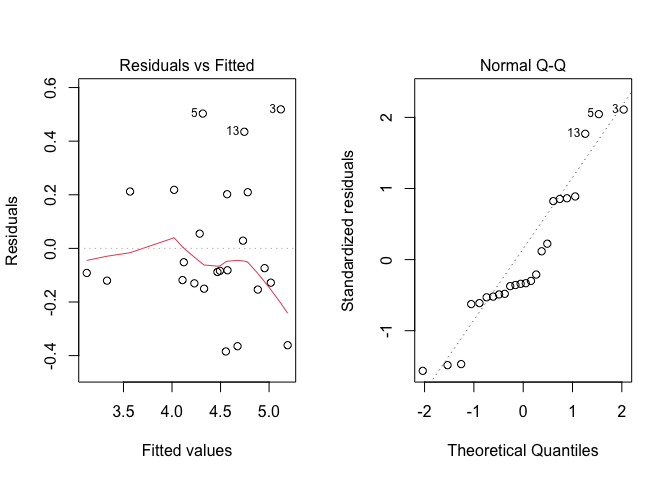
\includegraphics[width=0.9\linewidth]{_main_files/figure-latex/figName121-1} 

}

\caption{Analisi grafica dei residui per la prova di confronto erbicida}\label{fig:figName121}
\end{figure}

Dopo esserci rassicurati su questo importante aspetto, possiamo vedere che abbiamo due ipotesi nulle da testare (effetto dei trattamenti non significativo ed effetto dei blocchi non significativo), che possono essere entrambe rifiutate per P \textless{} 0.05.

Da questo punto in avanti, l'analisi procede come usuale, calcolando le medie marginali attese ed, eventualmente, confrontandole tra loro con una procedura di confronto multiplo, come descritto nei capitoli precedenti. Tener presente che, in questo esperimento, abbiamo 16 trattamenti, cioè \(16 \times 15 / 2 = 120\) confronti; di conseguenza, è opportuno operare la correzione per la molteplicità. Inoltre, dato che il trattamento più interessante è quello che rende massima la produzione, sarà opportuno ordinare le medie in senso decrescente, utilizzando l'argomento `reverse = T.'

\scriptsize

\begin{Shaded}
\begin{Highlighting}[]
\FunctionTok{library}\NormalTok{(emmeans)}
\NormalTok{medie }\OtherTok{\textless{}{-}} \FunctionTok{emmeans}\NormalTok{(mod, }\SpecialCharTok{\textasciitilde{}}\NormalTok{Code)}
\NormalTok{multcomp}\SpecialCharTok{::}\FunctionTok{cld}\NormalTok{(medie, }\AttributeTok{Letters =}\NormalTok{ LETTERS, }\AttributeTok{reverse =}\NormalTok{ T)}
\end{Highlighting}
\end{Shaded}

\begin{verbatim}
##  Code emmean   SE df lower.CL upper.CL .group
##  3      98.0 6.32 45    85.24    110.7  A    
##  10     97.0 6.32 45    84.26    109.7  A    
##  9      96.6 6.32 45    83.91    109.4  A    
##  1      95.4 6.32 45    82.67    108.1  A    
##  7      93.9 6.32 45    81.18    106.6  A    
##  2      91.6 6.32 45    78.84    104.3  A    
##  5      89.2 6.32 45    76.52    102.0  A    
##  14     89.0 6.32 45    76.24    101.7  A    
##  4      88.4 6.32 45    75.65    101.1  A    
##  6      84.7 6.32 45    71.94     97.4  A    
##  8      83.0 6.32 45    70.31     95.8  AB   
##  11     51.9 6.32 45    39.19     64.6   BC  
##  12     47.0 6.32 45    34.27     59.7    C  
##  16     35.7 6.32 45    22.99     48.4    C  
##  13     29.8 6.32 45    17.11     42.6    C  
##  15     21.9 6.32 45     9.13     34.6    C  
## 
## Results are averaged over the levels of: Block 
## Confidence level used: 0.95 
## P value adjustment: tukey method for comparing a family of 16 estimates 
## significance level used: alpha = 0.05
\end{verbatim}

\normalsize

Vi lascio il commento dei risultati come esercizio.

\hypertarget{disegni-a-quadrato-latino-1}{%
\section{Disegni a quadrato latino}\label{disegni-a-quadrato-latino-1}}

A volte i fattori di blocco sono più di uno e danno origine ad un disegno sperimentale detto `quadrato latino' di cui abbiamo parlato nel capitolo 3. Qui, forniremo un esempio tratto dalla pratica sperimentale industriale.

\hypertarget{caso-studio-confronto-tra-metodi-costruttivi}{%
\section{Caso studio: confronto tra metodi costruttivi}\label{caso-studio-confronto-tra-metodi-costruttivi}}

Immaginiamo di voler studiare il tempo necessario per costruire un componente elettronico, utilizzando quattro metodi diversi: è evidente che il tempo di costruzione sarà influenzato dalla perizia del tecnico e, per questo, utilizziamo quattro tecnici diversi, ad ognuno dei quali facciamo utilizzare tutti e quattro i metodi. Un esperimento così disegnato sarebbe a blocchi randomizzati, con il tecnico che fa da blocco per i trattamenti. Tuttavia, dobbiamo anche riconoscere che i quattro tecnici saranno via via meno efficienti, e quindi il metodo che utilizzeranno per primo sarà avvantaggiato, mentre quello che utilizzeranno per ultimo sarà svantaggiato. E'vero che i metodi sono assegnati in ordine random ad ogni tecnico, ma non si può comunque evitare che un metodo venga avvantaggiato rispetto ad un altro, perché, ad esempio, non viene mai ad occupare l'ultima posizione (o meglio, l'ultimo turno). Abbiamo già illustrato questa situazione in un capitolo precedente ed abbiamo visto come essa possa essere gestita imponendo un vincolo ulteriore alla randomizzazione e facendo in modo che ogni metodo occupi tutte e quattro i turni, in tecnici diversi. Il disegno è quindi a quadrato latino.

Il dataset dei risultati è disponibile online:

\begin{Shaded}
\begin{Highlighting}[]
\NormalTok{fileName }\OtherTok{\textless{}{-}} \StringTok{"https://www.casaonofri.it/\_datasets/Technicians.csv"}
\NormalTok{dataset }\OtherTok{\textless{}{-}} \FunctionTok{read.csv}\NormalTok{(fileName, }\AttributeTok{header=}\NormalTok{T)}
\NormalTok{dataset}
\end{Highlighting}
\end{Shaded}

\begin{verbatim}
##    Shift Technician Method Time
## 1      I     Andrew      C   90
## 2     II     Andrew      B   90
## 3    III     Andrew      A   89
## 4     IV     Andrew      D  104
## 5      I       Anna      D   96
## 6     II       Anna      C   91
## 7    III       Anna      B   97
## 8     IV       Anna      A  100
## 9      I    Michael      A   84
## 10    II    Michael      D   96
## 11   III    Michael      C   98
## 12    IV    Michael      B  104
## 13     I      Sarah      B   88
## 14    II      Sarah      A   88
## 15   III      Sarah      D   98
## 16    IV      Sarah      C  106
\end{verbatim}

\hypertarget{definizione-di-un-modello-lineare-2}{%
\section{Definizione di un modello lineare}\label{definizione-di-un-modello-lineare-2}}

In questo caso abbiamo un trattamento (metodo) e due effetti `blocco' (tecnico e turno) da includere nel modello, che può essere così definito:

\[Y_{ijk} = \mu + \gamma_k + \beta_j + \alpha_i + \varepsilon_{ijk}\]

dove \(\mu\) è l'intercetta, \(\gamma\) è l'effetto del turno k, \(\beta\) è l'effetto del tecnico j e \(\alpha\) è l'effetto del metodo i. L'elemento \(\varepsilon_{ijk}\) rappresenta la componente random individuale, di ogni osservazione e si assume normalmente distribuita, con media 0 e deviazione standard \(\sigma\).

Avendo già illustrato il processo di stima dei parametri e di scomposizione della varianza, quindi utilizziamo subito R per il `model fitting':

\begin{Shaded}
\begin{Highlighting}[]
\NormalTok{mod }\OtherTok{\textless{}{-}} \FunctionTok{lm}\NormalTok{(Time }\SpecialCharTok{\textasciitilde{}}\NormalTok{ Method }\SpecialCharTok{+}\NormalTok{ Technician}
          \SpecialCharTok{+}\NormalTok{ Shift, }\AttributeTok{data =}\NormalTok{ dataset)}
\end{Highlighting}
\end{Shaded}

Verifichiamo il rispetto delle assunzioni di base, con l'analisi grafica dei residui, riportata in Figura \ref{fig:figName122} (il codice è analogo a quello fornito più sopra).

\begin{figure}

{\centering 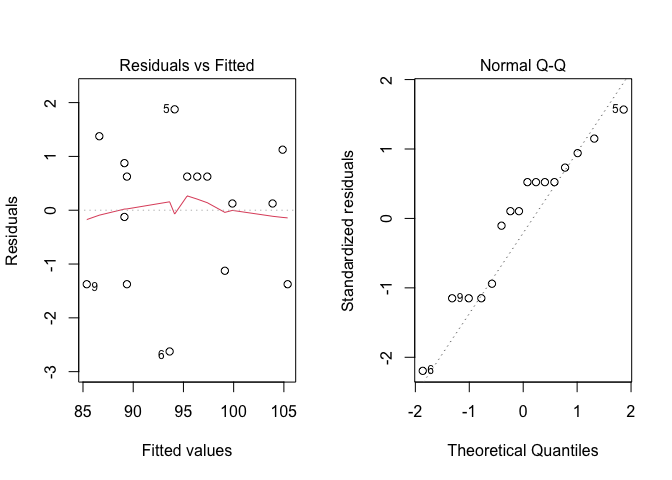
\includegraphics[width=0.9\linewidth]{_main_files/figure-latex/figName122-1} 

}

\caption{Analisi grafica dei residui per la prova di confronto tra metodi costruttivi}\label{fig:figName122}
\end{figure}

Non essendovi evidenti problemi, valutiamo la significatività degli effetti nel modello, analogamente a quanto abbiamo fatto nel caso dell'ANOVA a blocchi randomizzati. L'unica differenza sta nel fatto che, nei disegni a quadrato latino, vi sono tre effetti da testare, anche se l'unico ad avere una certa rilevanza è l'effetto del metodo di lavoro.

\begin{Shaded}
\begin{Highlighting}[]
\FunctionTok{anova}\NormalTok{(mod)}
\end{Highlighting}
\end{Shaded}

\begin{verbatim}
## Analysis of Variance Table
## 
## Response: Time
##            Df Sum Sq Mean Sq F value    Pr(>F)    
## Method      3 145.69  48.563 12.7377 0.0051808 ** 
## Technician  3  17.19   5.729  1.5027 0.3065491    
## Shift       3 467.19 155.729 40.8470 0.0002185 ***
## Residuals   6  22.87   3.812                      
## ---
## Signif. codes:  0 '***' 0.001 '**' 0.01 '*' 0.05 '.' 0.1 ' ' 1
\end{verbatim}

Vediamo che esiste una differenza significativa tra i metodi e l'ipotesi nulla può essere rifiutata con una bassissima probabilità di errore di prima specie.

Ovviamente, dopo aver eseguito un'ANOVA a blocchi randomizzati o a quadrato latino, andremo eventualmente ad eseguire un test di confronto multiplo, seguendo le raccomandazioni esposte nel capitolo precedente. Anche questa parte ve la lasciamo per esercizio.

\hypertarget{modelli-anova-a-due-vie}{%
\chapter{Modelli ANOVA a due vie}\label{modelli-anova-a-due-vie}}

Placeholder

\hypertarget{il-concetto-di-interazione}{%
\section{Il concetto di 'interazione'}\label{il-concetto-di-interazione}}

\hypertarget{tipi-di-interazione}{%
\section{Tipi di interazione}\label{tipi-di-interazione}}

\hypertarget{caso-studio-interazione-tra-lavorazioni-e-diserbo-chimico}{%
\section{Caso-studio: interazione tra lavorazioni e diserbo chimico}\label{caso-studio-interazione-tra-lavorazioni-e-diserbo-chimico}}

\hypertarget{definizione-del-modello-lineare}{%
\section{Definizione del modello lineare}\label{definizione-del-modello-lineare}}

\hypertarget{stima-dei-parametri-2}{%
\section{Stima dei parametri}\label{stima-dei-parametri-2}}

\hypertarget{verifica-delle-assunzioni-di-base}{%
\section{Verifica delle assunzioni di base}\label{verifica-delle-assunzioni-di-base}}

\hypertarget{scomposizione-delle-varianze}{%
\section{Scomposizione delle varianze}\label{scomposizione-delle-varianze}}

\hypertarget{medie-marginali-attese-1}{%
\section{Medie marginali attese}\label{medie-marginali-attese-1}}

\hypertarget{calcolo-degli-errori-standard-sem-e-sed}{%
\section{Calcolo degli errori standard (SEM e SED)}\label{calcolo-degli-errori-standard-sem-e-sed}}

\hypertarget{medie-marginali-attese-e-confronti-multipli-con-r}{%
\section{Medie marginali attese e confronti multipli con R}\label{medie-marginali-attese-e-confronti-multipli-con-r}}

\hypertarget{per-approfondire-un-po.}{%
\section{Per approfondire un po'\ldots.}\label{per-approfondire-un-po.}}

\hypertarget{anova-a-due-vie-scomposizione-manuale-della-varianza}{%
\subsection{Anova a due vie: scomposizione `manuale' della varianza}\label{anova-a-due-vie-scomposizione-manuale-della-varianza}}

\hypertarget{la-regressione-lineare-semplice}{%
\chapter{La regressione lineare semplice}\label{la-regressione-lineare-semplice}}

Placeholder

\hypertarget{caso-studio-effetto-della-concimazione-azotata-al-frumento}{%
\section{Caso studio: effetto della concimazione azotata al frumento}\label{caso-studio-effetto-della-concimazione-azotata-al-frumento}}

\hypertarget{analisi-preliminari}{%
\section{Analisi preliminari}\label{analisi-preliminari}}

\hypertarget{definizione-del-modello-lineare-1}{%
\section{Definizione del modello lineare}\label{definizione-del-modello-lineare-1}}

\hypertarget{stima-dei-parametri-3}{%
\section{Stima dei parametri}\label{stima-dei-parametri-3}}

\hypertarget{valutazione-della-bontuxe0-del-modello}{%
\section{Valutazione della bontà del modello}\label{valutazione-della-bontuxe0-del-modello}}

\hypertarget{valutazione-grafica}{%
\subsection{Valutazione grafica}\label{valutazione-grafica}}

\hypertarget{errori-standard-dei-parametri}{%
\subsection{Errori standard dei parametri}\label{errori-standard-dei-parametri}}

\hypertarget{test-f-per-la-mancanza-dadattamento}{%
\subsection{Test F per la mancanza d'adattamento}\label{test-f-per-la-mancanza-dadattamento}}

\hypertarget{test-f-per-la-bontuxe0-di-adattamento-e-coefficiente-di-determinazione}{%
\subsection{Test F per la bontà di adattamento e coefficiente di determinazione}\label{test-f-per-la-bontuxe0-di-adattamento-e-coefficiente-di-determinazione}}

\hypertarget{previsioni}{%
\section{Previsioni}\label{previsioni}}

\hypertarget{per-approfondire-un-po-1}{%
\section{Per approfondire un po'\ldots{}}\label{per-approfondire-un-po-1}}

\hypertarget{la-regressione-non-lineare}{%
\chapter{La regressione non-lineare}\label{la-regressione-non-lineare}}

Placeholder

\hypertarget{caso-studio-degradazione-di-un-erbicida-nel-terreno}{%
\section{Caso studio: degradazione di un erbicida nel terreno}\label{caso-studio-degradazione-di-un-erbicida-nel-terreno}}

\hypertarget{scelta-della-funzione}{%
\section{Scelta della funzione}\label{scelta-della-funzione}}

\hypertarget{stima-dei-parametri-4}{%
\section{Stima dei parametri}\label{stima-dei-parametri-4}}

\hypertarget{linearizzazione-della-funzione}{%
\subsection{Linearizzazione della funzione}\label{linearizzazione-della-funzione}}

\hypertarget{approssimazione-della-vera-funzione-tramite-una-polinomiale-in-x}{%
\subsection{Approssimazione della vera funzione tramite una polinomiale in X}\label{approssimazione-della-vera-funzione-tramite-una-polinomiale-in-x}}

\hypertarget{minimi-quadrati-non-lineari}{%
\subsection{Minimi quadrati non-lineari}\label{minimi-quadrati-non-lineari}}

\hypertarget{la-regressione-non-lineare-con-r}{%
\section{La regressione non-lineare con R}\label{la-regressione-non-lineare-con-r}}

\hypertarget{verifica-della-bontuxe0-del-modello}{%
\section{Verifica della bontà del modello}\label{verifica-della-bontuxe0-del-modello}}

\hypertarget{analisi-grafica-dei-residui-1}{%
\subsection{Analisi grafica dei residui}\label{analisi-grafica-dei-residui-1}}

\hypertarget{test-f-per-la-mancanza-di-adattamento-approssimato}{%
\subsection{Test F per la mancanza di adattamento (approssimato)}\label{test-f-per-la-mancanza-di-adattamento-approssimato}}

\hypertarget{errori-standard-dei-parametri-1}{%
\subsection{Errori standard dei parametri}\label{errori-standard-dei-parametri-1}}

\hypertarget{coefficienti-di-determinazione}{%
\subsection{Coefficienti di determinazione}\label{coefficienti-di-determinazione}}

\hypertarget{funzioni-lineari-e-nonlineari-dei-parametri}{%
\section{Funzioni lineari e nonlineari dei parametri}\label{funzioni-lineari-e-nonlineari-dei-parametri}}

\hypertarget{previsioni-1}{%
\section{Previsioni}\label{previsioni-1}}

\hypertarget{gestione-delle-situazioni-patologiche}{%
\section{Gestione delle situazioni `patologiche'}\label{gestione-delle-situazioni-patologiche}}

\hypertarget{trasformazione-del-modello}{%
\subsection{Trasformazione del modello}\label{trasformazione-del-modello}}

\hypertarget{trasformazione-dei-dati}{%
\subsection{Trasformazione dei dati}\label{trasformazione-dei-dati}}

\hypertarget{per-approfondire-un-po-2}{%
\section{Per approfondire un po'\ldots{}}\label{per-approfondire-un-po-2}}

\hypertarget{riparametrizzazione-delle-funzioni-non-lineari}{%
\subsection{Riparametrizzazione delle funzioni non-lineari}\label{riparametrizzazione-delle-funzioni-non-lineari}}

\hypertarget{altre-letture-9}{%
\subsection{Altre letture}\label{altre-letture-9}}

\hypertarget{esercizi}{%
\chapter{Esercizi}\label{esercizi}}

Placeholder

\hypertarget{capitoli-1-e-2}{%
\section{Capitoli 1 e 2}\label{capitoli-1-e-2}}

\hypertarget{esercizio-1}{%
\subsection{Esercizio 1}\label{esercizio-1}}

\hypertarget{capitolo-3}{%
\section{Capitolo 3}\label{capitolo-3}}

\hypertarget{esercizio-1-1}{%
\subsection{Esercizio 1}\label{esercizio-1-1}}

\hypertarget{esercizio-2}{%
\subsection{Esercizio 2}\label{esercizio-2}}

\hypertarget{esercizio-3}{%
\subsection{Esercizio 3}\label{esercizio-3}}

\hypertarget{capitolo-4}{%
\section{Capitolo 4}\label{capitolo-4}}

\hypertarget{esercizio-1-2}{%
\subsection{Esercizio 1}\label{esercizio-1-2}}

\hypertarget{esercizio-2-1}{%
\subsection{Esercizio 2}\label{esercizio-2-1}}

\hypertarget{esercizio-3-1}{%
\subsection{Esercizio 3}\label{esercizio-3-1}}

\hypertarget{esercizio-4}{%
\subsection{Esercizio 4}\label{esercizio-4}}

\hypertarget{esercizio-5}{%
\subsection{Esercizio 5}\label{esercizio-5}}

\hypertarget{esercizio-6}{%
\subsection{Esercizio 6}\label{esercizio-6}}

\hypertarget{esercizio-7}{%
\subsection{Esercizio 7}\label{esercizio-7}}

\hypertarget{esercizio-8}{%
\subsection{Esercizio 8}\label{esercizio-8}}

\hypertarget{capitolo-5}{%
\section{Capitolo 5}\label{capitolo-5}}

\hypertarget{esercizio-1-3}{%
\subsection{Esercizio 1}\label{esercizio-1-3}}

\hypertarget{esercizio-2-2}{%
\subsection{Esercizio 2}\label{esercizio-2-2}}

\hypertarget{esercizio-3-2}{%
\subsection{Esercizio 3}\label{esercizio-3-2}}

\hypertarget{esercizio-4-1}{%
\subsection{Esercizio 4}\label{esercizio-4-1}}

\hypertarget{esercizio-5-1}{%
\subsection{Esercizio 5}\label{esercizio-5-1}}

\hypertarget{capitolo-6}{%
\section{Capitolo 6}\label{capitolo-6}}

\hypertarget{esercizio-1-4}{%
\subsection{Esercizio 1}\label{esercizio-1-4}}

\hypertarget{esercizio-2-3}{%
\subsection{Esercizio 2}\label{esercizio-2-3}}

\hypertarget{esercizio-3-3}{%
\subsection{Esercizio 3}\label{esercizio-3-3}}

\hypertarget{esercizio-4-2}{%
\subsection{Esercizio 4}\label{esercizio-4-2}}

\hypertarget{esercizio-5-2}{%
\subsection{Esercizio 5}\label{esercizio-5-2}}

\hypertarget{esercizio-6-1}{%
\subsection{Esercizio 6}\label{esercizio-6-1}}

\hypertarget{esercizio-7-1}{%
\subsection{Esercizio 7}\label{esercizio-7-1}}

\hypertarget{esercizio-8-1}{%
\subsection{Esercizio 8}\label{esercizio-8-1}}

\hypertarget{esercizio-9}{%
\subsection{Esercizio 9}\label{esercizio-9}}

\hypertarget{esercizio-10}{%
\subsection{Esercizio 10}\label{esercizio-10}}

\hypertarget{capitoli-da-7-a-9}{%
\section{Capitoli da 7 a 9}\label{capitoli-da-7-a-9}}

\hypertarget{esercizio-1-5}{%
\subsection{Esercizio 1}\label{esercizio-1-5}}

\hypertarget{esercizio-2-4}{%
\subsection{Esercizio 2}\label{esercizio-2-4}}

\hypertarget{esercizio-3-4}{%
\subsection{Esercizio 3}\label{esercizio-3-4}}

\hypertarget{esercizio-4-3}{%
\subsection{Esercizio 4}\label{esercizio-4-3}}

\hypertarget{capitolo-10}{%
\section{Capitolo 10}\label{capitolo-10}}

\hypertarget{esercizio-1-6}{%
\subsection{Esercizio 1}\label{esercizio-1-6}}

\hypertarget{esercizio-2-5}{%
\subsection{Esercizio 2}\label{esercizio-2-5}}

\hypertarget{esercizio-3-5}{%
\subsection{Esercizio 3}\label{esercizio-3-5}}

\hypertarget{capitoli-11-e-12}{%
\section{Capitoli 11 e 12}\label{capitoli-11-e-12}}

\hypertarget{esercizio-1-7}{%
\subsection{Esercizio 1}\label{esercizio-1-7}}

\hypertarget{esercizio-2-6}{%
\subsection{Esercizio 2}\label{esercizio-2-6}}

\hypertarget{esercizio-3-6}{%
\subsection{Esercizio 3}\label{esercizio-3-6}}

\hypertarget{esercizio-4-4}{%
\subsection{Esercizio 4}\label{esercizio-4-4}}

\hypertarget{esercizio-5-3}{%
\subsection{Esercizio 5}\label{esercizio-5-3}}

\hypertarget{esercizio-6-2}{%
\subsection{Esercizio 6}\label{esercizio-6-2}}

\hypertarget{capitolo-13}{%
\section{Capitolo 13}\label{capitolo-13}}

\hypertarget{esercizio-1-8}{%
\subsection{Esercizio 1}\label{esercizio-1-8}}

\hypertarget{esercizio-2-7}{%
\subsection{Esercizio 2}\label{esercizio-2-7}}

\hypertarget{capitolo-14}{%
\section{Capitolo 14}\label{capitolo-14}}

\hypertarget{esercizio-1-9}{%
\subsection{Esercizio 1}\label{esercizio-1-9}}

\hypertarget{esercizio-2-8}{%
\subsection{Esercizio 2}\label{esercizio-2-8}}

\hypertarget{esercizio-3-7}{%
\subsection{Esercizio 3}\label{esercizio-3-7}}

\hypertarget{esercizio-4-5}{%
\subsection{Esercizio 4}\label{esercizio-4-5}}

\hypertarget{esercizio-5-4}{%
\subsection{Esercizio 5}\label{esercizio-5-4}}

\hypertarget{esercizio-6-3}{%
\subsection{Esercizio 6}\label{esercizio-6-3}}

\hypertarget{esercizio-7-2}{%
\subsection{Esercizio 7}\label{esercizio-7-2}}

\hypertarget{appendice-1-breve-introduzione-ad-r}{%
\chapter{Appendice 1: breve introduzione ad R}\label{appendice-1-breve-introduzione-ad-r}}

Placeholder

\hypertarget{cosa-uxe8-r}{%
\section*{Cosa è R?}\label{cosa-uxe8-r}}
\addcontentsline{toc}{section}{Cosa è R?}

\hypertarget{oggetti-e-assegnazioni}{%
\section*{Oggetti e assegnazioni}\label{oggetti-e-assegnazioni}}
\addcontentsline{toc}{section}{Oggetti e assegnazioni}

\hypertarget{costanti-e-vettori}{%
\subsection*{Costanti e vettori}\label{costanti-e-vettori}}
\addcontentsline{toc}{subsection}{Costanti e vettori}

\hypertarget{matrici}{%
\subsection*{Matrici}\label{matrici}}
\addcontentsline{toc}{subsection}{Matrici}

\hypertarget{dataframe}{%
\subsection*{Dataframe}\label{dataframe}}
\addcontentsline{toc}{subsection}{Dataframe}

\hypertarget{quale-oggetto-sto-utilizzando}{%
\subsection*{Quale oggetto sto utilizzando?}\label{quale-oggetto-sto-utilizzando}}
\addcontentsline{toc}{subsection}{Quale oggetto sto utilizzando?}

\hypertarget{operazioni-ed-operatori}{%
\section*{Operazioni ed operatori}\label{operazioni-ed-operatori}}
\addcontentsline{toc}{section}{Operazioni ed operatori}

\hypertarget{funzioni-ed-argomenti}{%
\section*{Funzioni ed argomenti}\label{funzioni-ed-argomenti}}
\addcontentsline{toc}{section}{Funzioni ed argomenti}

\hypertarget{consigli-per-limmissione-di-dati-sperimentali}{%
\section*{Consigli per l'immissione di dati sperimentali}\label{consigli-per-limmissione-di-dati-sperimentali}}
\addcontentsline{toc}{section}{Consigli per l'immissione di dati sperimentali}

\hypertarget{immissione-di-numeri-progressivi}{%
\subsection*{Immissione di numeri progressivi}\label{immissione-di-numeri-progressivi}}
\addcontentsline{toc}{subsection}{Immissione di numeri progressivi}

\hypertarget{immissione-dei-codici-delle-tesi-e-dei-blocchi}{%
\subsection*{Immissione dei codici delle tesi e dei blocchi}\label{immissione-dei-codici-delle-tesi-e-dei-blocchi}}
\addcontentsline{toc}{subsection}{Immissione dei codici delle tesi e dei blocchi}

\hypertarget{immissione-dei-valori-e-creazione-del-datframe}{%
\subsection*{Immissione dei valori e creazione del datframe}\label{immissione-dei-valori-e-creazione-del-datframe}}
\addcontentsline{toc}{subsection}{Immissione dei valori e creazione del datframe}

\hypertarget{leggere-e-salvare-dati-esterni}{%
\subsection*{Leggere e salvare dati esterni}\label{leggere-e-salvare-dati-esterni}}
\addcontentsline{toc}{subsection}{Leggere e salvare dati esterni}

\hypertarget{alcune-operazioni-comuni-sul-dataset}{%
\section*{Alcune operazioni comuni sul dataset}\label{alcune-operazioni-comuni-sul-dataset}}
\addcontentsline{toc}{section}{Alcune operazioni comuni sul dataset}

\hypertarget{selezionare-un-subset-di-dati}{%
\subsection*{Selezionare un subset di dati}\label{selezionare-un-subset-di-dati}}
\addcontentsline{toc}{subsection}{Selezionare un subset di dati}

\hypertarget{ordinare-un-vettore-o-un-dataframe}{%
\subsection*{Ordinare un vettore o un dataframe}\label{ordinare-un-vettore-o-un-dataframe}}
\addcontentsline{toc}{subsection}{Ordinare un vettore o un dataframe}

\hypertarget{workspace}{%
\section*{Workspace}\label{workspace}}
\addcontentsline{toc}{section}{Workspace}

\hypertarget{script-o-programmi}{%
\section*{Script o programmi}\label{script-o-programmi}}
\addcontentsline{toc}{section}{Script o programmi}

\hypertarget{interrogazione-di-oggetti}{%
\section*{Interrogazione di oggetti}\label{interrogazione-di-oggetti}}
\addcontentsline{toc}{section}{Interrogazione di oggetti}

\hypertarget{altre-funzioni-matriciali}{%
\section*{Altre funzioni matriciali}\label{altre-funzioni-matriciali}}
\addcontentsline{toc}{section}{Altre funzioni matriciali}

\hypertarget{cenni-sulle-funzionalituxe0-grafiche-in-r}{%
\section*{Cenni sulle funzionalità grafiche in R}\label{cenni-sulle-funzionalituxe0-grafiche-in-r}}
\addcontentsline{toc}{section}{Cenni sulle funzionalità grafiche in R}

\hypertarget{altre-letture-10}{%
\section*{Altre letture}\label{altre-letture-10}}
\addcontentsline{toc}{section}{Altre letture}


\end{document}
